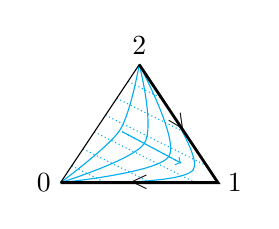
\begin{tikzpicture}
\node[above] (c) at (1,1.5) {$2$};
\node[left]  (a) at (0,0) {$0$};
\node[right] (b) at (2,0) {$1$};

%  for t \in [0,1] : (t,1.5)  --  (4*t ,0) if t < .5 else (3-2*t, 3*(t-.5))  
\draw[cyan, densely dotted] (0.143, 0.214) -- (0.571, 0.000);
\draw[cyan, densely dotted] (0.286, 0.429) -- (1.143, 0.000);
\draw[cyan, densely dotted] (0.429, 0.643) -- (1.714, 0.000);
\draw[cyan, densely dotted] (0.571, 0.857) -- (1.857, 0.214);
\draw[cyan, densely dotted] (0.714, 1.071) -- (1.571, 0.643);
\draw[cyan, densely dotted] (0.857, 1.286) -- (1.286, 1.071);

% a=.488, t=.2,.4,.6,.8: (2-(cos(a)*2)*t*cos(a), (cos(a)*2)*t*sin(a))
\draw [cyan] plot [smooth] coordinates { (0,0) (1.687, 0.165) (1,1.5)};
\draw [cyan] plot [smooth] coordinates { (0,0) (1.375, 0.331) (1,1.5)};
\draw [cyan] plot [smooth] coordinates { (0,0) (1.063, 0.496) (1,1.5)};
\draw [cyan] plot [smooth] coordinates { (0,0) (0.751, 0.662) (1,1.5)};

% t=.3 to t=.78
\draw[cyan, -to] (0.783, 0.647) -- (1.532, 0.248);

\draw[cyan, dotted] (0.783, 0.647) -- (1.532, 0.248);

\draw[line width=1px] (0,0) 
    -- (2,0)    node[sloped, scale=.9, pos=0.5, xscale=-1] {$>$} 
%                node[scale=1, pos=0.5, below] {$I_{0,1}$} 
    -- (1,1.5)  node[sloped, scale=.9, pos=0.5] {$>$};
%                node[scale=1, pos=0.5, above right] {$I_{1,2}$};

\draw (0,0) -- (1,1.5);

\end{tikzpicture}
